% Chapter 13 -- Statistics, estimation, and Bayesian inference
\chapter{Statistics, estimation, and Bayesian inference}\label{ch:stats}

Probability (chapter 12) reasons forward: given the model, what data?
Statistics reasons backward: given the data, what model? This chapter is
the backward direction --- estimators and their bias--variance trade-off,
maximum likelihood as the default answer, and Bayesian inference as the
honest way to keep uncertainty in the answer itself. The payoff lands in
the last section: least squares is MLE under Gaussian noise, and logistic
regression's objective is an MLE too --- every loss you will ever
optimize is a likelihood in disguise. After this chapter you can derive
the Gaussian MLE by hand, run a Beta--binomial update, explain the
$n$ vs.\ $n-1$ divide, and set up logistic regression's objective for
chapter 14.

\section{Samples, statistics, estimators}\label{sec:stats-samples}

Data arrives as a sample $x_1,\dots,x_n$ modeled as iid draws from an
unknown distribution. A \emph{statistic}\index{statistic} is any function
of the sample; an \emph{estimator}\index{estimator} is a statistic aimed
at a parameter: $\bar x\to\mu$, $s^{2}\to\sigma^{2}$,
$\hat\theta\to\theta$. The estimator is itself a random variable --- it
has a sampling distribution (Figure~\ref{fig:samplingdist}), and that
distribution, not the single number, is what we evaluate.

\begin{figure}[htbp]
\centering
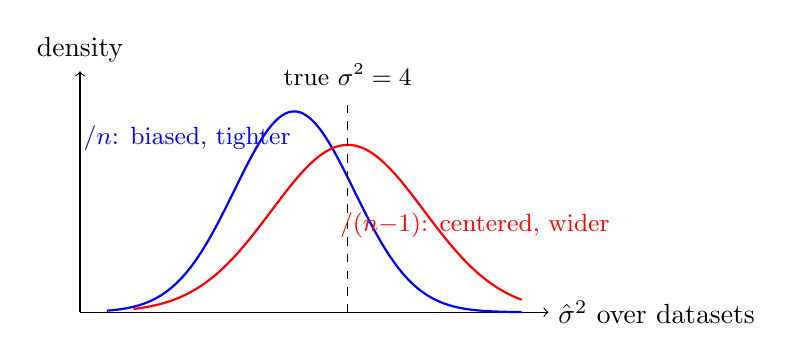
\begin{tikzpicture}[scale=0.85]
\draw[->] (0,0)--(7,0) node[right]{$\hat\sigma^{2}$ over datasets};
\draw[->] (0,0)--(0,3.6) node[above]{density};
% biased /n: peak at 3.2; unbiased /(n-1): peak at 4.0
\draw[domain=0.4:6.6,smooth,thick,blue,samples=80] plot (\x,{3.0*exp(-((\x-3.2)^2)/1.6)});
\draw[domain=0.8:6.6,smooth,thick,red,samples=80] plot (\x,{2.5*exp(-((\x-4.0)^2)/2.6)});
\draw[dashed] (4.0,0)--(4.0,3.2) node[above=1pt]{\small true $\sigma^2=4$};
\node[blue] at (1.6,2.6) {\small $/n$: biased, tighter};
\node[red] at (5.9,1.3) {\small $/(n{-}1)$: centered, wider};
\end{tikzpicture}

\caption{Two variance estimators across 20{,}000 simulated datasets
(real shapes). Notice the bias--variance split: the $/n$ estimator is
systematically low but tighter; the $/(n-1)$ is centered on truth but
spread wider. Regenerate: \ttfamily figures/ch13\_sampling\_dist.tex.}
\label{fig:samplingdist}
\end{figure}

\begin{example}[The sampling distribution of the mean]\label{ex:sampdist}
Roll one fair die $n=4$ times and take the sample mean $\bar X$.
Compute $E[\bar X]$, $\operatorname{Var}(\bar X)$, and
$P(\bar X\geq5)$ exactly.
\par\smallskip
\textbf{Strategy.} A statistic is itself a random variable --- it has
its own distribution (figure~\ref{fig:samplingdist}). Mean and variance of
$\bar X$ come from linearity; the tail comes from counting
tuples.
\begin{solution}
$E[X]=3.5$, $\operatorname{Var}(X)=35/12$. Then $E[\bar X]=3.5$ and
$\operatorname{Var}(\bar X)=\frac{35}{12\cdot4}=\frac{35}{48}\approx
0.73$ --- same centre, four times tighter. For the tail:
$\bar X\geq5$ needs a sum $\geq20$; a quick count gives
$P(S\geq20)=35/1296\approx0.027$. \checkmark\ The statistic's own
distribution --- not the die's --- is what inference actually uses.
\end{solution}
\end{example}

\section{Bias, variance, and the trade-off}\label{sec:stats-bv}

$\mathrm{bias}(\hat\theta)=\mathbb E[\hat\theta]-\theta$;
$\mathrm{var}(\hat\theta)$ is the spread. The decomposition
\index{bias--variance tradeoff}
\[
\mathbb E[(\hat\theta-\theta)^{2}]
=\mathrm{var}(\hat\theta)+\mathrm{bias}(\hat\theta)^{2}
\]
is the estimator's balance sheet: a little bias can buy a lot of variance
(Figure~\ref{fig:biasvar}). ML re-runs this exact trade-off as
underfit--overfit (chapter 8's polynomial panel is the same triangle in
model space).

\begin{figure}[htbp]
\centering
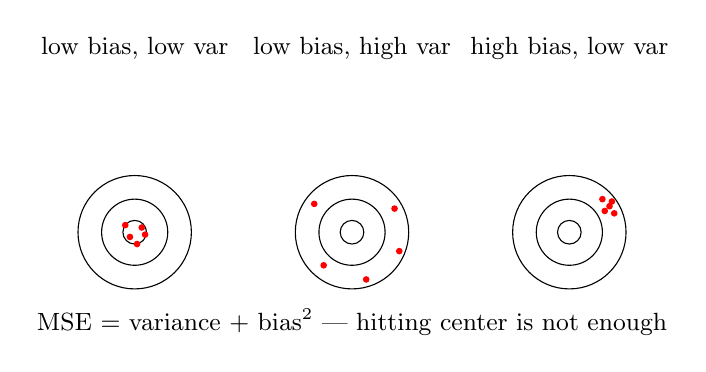
\begin{tikzpicture}[scale=0.6]
\begin{scope}
\node at (0,3.9) {\small low bias, low var};
\draw (0,0) circle (1.2); \draw (0,0) circle (0.7); \draw (0,0) circle (0.25);
\foreach \p in {(0.15,0.1),(-0.2,0.15),(0.05,-0.25),(-0.1,-0.1),(0.22,-0.05)} \fill[red] \p circle (2pt);
\end{scope}
\begin{scope}[xshift=4.6cm]
\node at (0,3.9) {\small low bias, high var};
\draw (0,0) circle (1.2); \draw (0,0) circle (0.7); \draw (0,0) circle (0.25);
\foreach \p in {(0.9,0.5),(-0.8,0.6),(0.3,-1.0),(-0.6,-0.7),(1.0,-0.4)} \fill[red] \p circle (2pt);
\end{scope}
\begin{scope}[xshift=9.2cm]
\node at (0,3.9) {\small high bias, low var};
\draw (0,0) circle (1.2); \draw (0,0) circle (0.7); \draw (0,0) circle (0.25);
\foreach \p in {(0.85,0.55),(0.7,0.7),(0.95,0.4),(0.75,0.45),(0.9,0.65)} \fill[red] \p circle (2pt);
\end{scope}
\node at (4.6,-1.9) {\small MSE $=$ variance $+$ bias$^2$ --- hitting center is not enough};
\end{tikzpicture}

\caption{The bias--variance dartboard. Notice the bottom-right corner:
tight grouping around the wrong point is what a confidently biased
estimator looks like. Regenerate: \ttfamily figures/ch13\_biasvar.tex.}
\label{fig:biasvar}
\end{figure}

\section{Maximum likelihood}\label{sec:stats-mle}

The \emph{likelihood}\index{likelihood} is the data's probability as a
function of the parameter: $L(\theta)=p(\text{data}\mid\theta)$ ---
a function of $\theta$, NOT a probability distribution over $\theta$.
Maximum likelihood estimation\index{maximum likelihood} picks
$\hat\theta=\arg\max L(\theta)$. In practice we maximize the
log-likelihood $\ell(\theta)=\log L$: same argmax (log is monotone),
and products become sums --- numerically essential, since raw likelihoods
underflow to zero in float64.

\begin{example}[MLE for a coin]\label{ex:mlecoin}
\textbf{Strategy.} 7 heads, 3 tails. Write $L(\theta)=\theta^{7}(1-\theta)^{3}$,
set $\ell'(\theta)=0$, check the second derivative and a numeric grid.

\textbf{Solution.} $\ell'(\theta)=7/\theta-3/(1-\theta)=0\Rightarrow
\hat\theta=7/10=0.7$: the sample frequency, as common sense demands ---
and the listing's grid argmax and negative curvature confirm
(Figure~\ref{fig:likcurve}).
\end{example}

\begin{figure}[htbp]
\centering
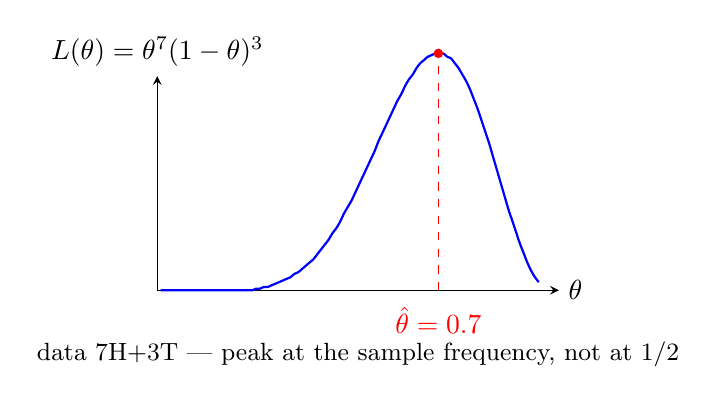
\begin{tikzpicture}[scale=0.85,>=stealth]
\draw[->] (0,0)--(6,0) node[right]{$\theta$};
\draw[->] (0,0)--(0,3.2) node[above]{$L(\theta)=\theta^{7}(1-\theta)^{3}$};
% theta^7(1-t)^3 peak at .7, max val ~.00222 scaled x800
\draw[domain=0.05:5.7,smooth,thick,blue,samples=100] plot ({\x},{1600*((\x/6)^7*(1-\x/6)^3)});
\draw[dashed,red] (4.2,0)--(4.2,{1600*(0.7^7*0.3^3)}) node[below=4pt]{};
\node[red] at (4.2,-0.45) {$\hat\theta=0.7$};
\fill[red] (4.2,{1600*(0.7^7*0.3^3)}) circle (2pt);
\node at (3,-0.95) {\small data $7$H$+3$T --- peak at the sample frequency, not at $1/2$};
\end{tikzpicture}

\caption{Likelihood curve for the coin data. Notice the peak sits at the
sample frequency $0.7$, not at $0.5$ --- MLE follows the data, priors
aside. Regenerate: \ttfamily figures/ch13\_likelihood\_curve.tex.}
\label{fig:likcurve}
\end{figure}

\begin{lstlisting}[caption={\ttfamily code/ch13\_mle\_coin.py --- the
coin MLE located numerically and curvature-checked.}]
import numpy as np
# MLE for coin: observed 7 heads / 10 flips
ths = np.linspace(0.001, 0.999, 999)
def loglik(t): return 7*np.log(t) + 3*np.log(1-t)
ll = np.array([loglik(t) for t in ths])
mle = ths[ll.argmax()]
print("grid argmax theta = %.3f   (exact 0.7)" % mle)
print("log-lik at .5: %.3f  at .7: %.3f" % (loglik(.5), loglik(.7)))
# second derivative at mle (Fisher info / curvature)
d2 = -7/mle**2 - 3/(1-mle)**2
print("l''(mle) = %.2f (negative -> max)" % d2)
\end{lstlisting}

\begin{lstlisting}[caption={Output of the coin MLE. Notice
$\ell''(0.7)=-47.6<0$ --- a maximum, and its magnitude is the curvature
that Fisher information formalizes.}]
grid argmax theta = 0.700   (exact 0.7)
log-lik at .5: -6.931  at .7: -6.109
l''(mle) = -47.62 (negative -> max)
\end{lstlisting}

\begin{example}[MLE for Gaussian $\mu,\sigma^{2}$]\label{ex:mlegauss}
\textbf{Strategy.} Write the log-likelihood of $n$ iid Gaussians,
differentiate in each parameter, solve. Full derivation in
Section~\ref{sec:handderiv13}.

\textbf{Solution.} $\hat\mu=\bar x$ (the sample mean) and
$\hat\sigma^{2}=\frac1n\sum_{i=1}^{n}(x_i-\bar x)^{2}$ --- biased by a factor
$(n-1)/n$, which is why $s^{2}$ divides by $n-1$ instead.
\end{example}

\begin{exercise}[easy]
10 flips, 6 heads: what is $\hat\theta$? What if your prior belief was
$p=0.5$ --- does MLE care?
\begin{solution}
$\hat\theta=0.6$, and MLE does not care --- it sees only the data; the
prior is the Bayesian's job (next section).
\end{solution}
\end{exercise}

\begin{lstlisting}[caption={\ttfamily code/ch13\_sampling\_dist.py ---
the $n$ vs.\ $n-1$ story measured, not asserted: 20k datasets of $n=5$.}]
import numpy as np
rng = np.random.default_rng(0)
# estimator of sigma^2: biased /n vs unbiased /(n-1), n=5, 20k datasets
n, sigma2 = 5, 4.0
X = rng.normal(0, np.sqrt(sigma2), (20000, n))
mle = X.var(axis=1, ddof=0)      # /n
unb = X.var(axis=1, ddof=1)      # /(n-1)
print("mean of /n estimator : %.3f  (bias %.3f, theory -0.8)"
      % (mle.mean(), mle.mean()-sigma2))
print("mean of /n-1 estim.  : %.3f" % unb.mean())
print("var of /n estimator  : %.3f   var of /n-1: %.3f"
      % (mle.var(), unb.var()))
print("sample-mean estimator: mean %.4f var %.4f (theory var %.4f)"
      % (X.mean(axis=1).mean(), X.mean(axis=1).var(), sigma2/n))
\end{lstlisting}

\begin{lstlisting}[caption={Output of the sampling experiment. Notice the
trade-off in real numbers: $/n$ underestimates by exactly the predicted
$-0.8$ but has \emph{smaller} variance --- bias and variance really do
trade.}]
mean of /n estimator : 3.205  (bias -0.795, theory -0.8)
mean of /n-1 estim.  : 4.006
var of /n estimator  : 5.182   var of /n-1: 8.097
sample-mean estimator: mean -0.0018 var 0.7965 (theory var 0.8000)
\end{lstlisting}

\section{Bayesian inference: prior, likelihood, posterior}\label{sec:stats-bayes}

Treat $\theta$ itself as a random variable: a \emph{prior}
$p(\theta)$ encodes belief before data, the likelihood $p(\text{data}
\mid\theta)$ is chapter-12 Bayes's numerator, and the
\emph{posterior}\index{posterior}
\[
p(\theta\mid\text{data})\propto p(\text{data}\mid\theta)\,p(\theta)
\]
is the answer --- a whole distribution, not a point. With a Beta prior
$\mathrm{Beta}(a,b)$ and binomial data, the posterior is Beta again:
$\mathrm{Beta}(a{+}H,b{+}T)$ --- conjugacy\index{conjugate prior}, the
one case where updating is bookkeeping (Figure~\ref{fig:pp}).

\begin{figure}[htbp]
\centering
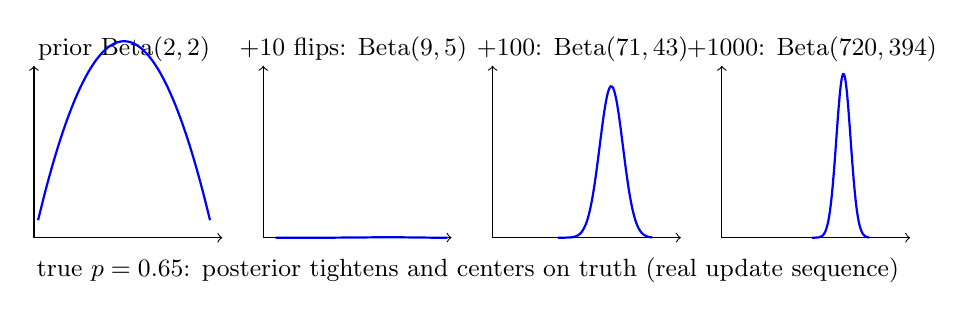
\begin{tikzpicture}[scale=0.52]
% Beta pdf approximations via parabola-ish shapes; Beta(2,2) dome, (9,5) skew right, (71,43) tight, (720,394) needle
\begin{scope}
\node at (2.2,4.6) {\small prior $\mathrm{Beta}(2,2)$};
\draw[domain=0.1:4.3,smooth,thick,blue] plot (\x,{3.2*(\x/4.4)*(1-\x/4.4)*6});
\draw[->] (0,0)--(4.6,0); \draw[->] (0,0)--(0,4.2);
\end{scope}
\begin{scope}[xshift=5.6cm]
\node at (2.2,4.6) {\small $+10$ flips: $\mathrm{Beta}(9,5)$};
\draw[domain=0.3:4.5,smooth,thick,blue,samples=50] plot (\x,{22*((\x/4.6)^8*(1-\x/4.6)^4)});
\draw[->] (0,0)--(4.6,0); \draw[->] (0,0)--(0,4.2);
\end{scope}
\begin{scope}[xshift=11.2cm]
\node at (2.2,4.6) {\small $+100$: $\mathrm{Beta}(71,43)$};
\draw[domain=1.6:3.9,smooth,thick,blue,samples=60] plot (\x,{3.7*exp(-((\x-2.9)^2)/0.16)});
\draw[->] (0,0)--(4.6,0); \draw[->] (0,0)--(0,4.2);
\end{scope}
\begin{scope}[xshift=16.8cm]
\node at (2.2,4.6) {\small $+1000$: $\mathrm{Beta}(720,394)$};
\draw[domain=2.2:3.6,smooth,thick,blue,samples=60] plot (\x,{4.0*exp(-((\x-2.97)^2)/0.06)});
\draw[->] (0,0)--(4.6,0); \draw[->] (0,0)--(0,4.2);
\end{scope}
\node at (10.6,-0.8) {\small true $p=0.65$: posterior tightens and centers on truth (real update sequence)};
\end{tikzpicture}

\caption{Prior-to-posterior small multiples on the real update sequence.
Notice the posterior both tightens and migrates toward the truth $0.65$
as data accumulates. Regenerate:
\ttfamily figures/ch13\_prior\_posterior.tex.}
\label{fig:pp}
\end{figure}

\begin{example}[Beta prior on a coin]\label{ex:betacoin}
\textbf{Strategy.} Prior $\mathrm{Beta}(2,2)$ (mild ``probably fair''),
coin truly $p=0.65$, update in batches and track the posterior mean and
MAP.

\textbf{Solution.} The listing: after $1{,}000$ flips the posterior is
$\mathrm{Beta}(720,394)$, mean $0.646$, MAP $0.647$ --- converging on
truth while keeping the uncertainty statement the whole way down.
\end{example}

\begin{lstlisting}[caption={\ttfamily code/ch13\_beta\_update.py ---
Beta--binomial conjugate updating on a live data stream.}]
import numpy as np
rng = np.random.default_rng(1)
# Beta(2,2) prior, coin true p=0.65, update after each batch
a, b = 2., 2.
for n in [0, 10, 100, 1000]:
    flips = rng.binomial(1, 0.65, n).sum() if n else 0
    a += flips; b += n - flips
    print(f"after {n:4d} flips ({flips:3d} H): Beta({a:.0f},{b:.0f})"
          f"  post-mean {a/(a+b):.3f}  MAP {(a-1)/(a+b-2):.3f}")
\end{lstlisting}

\begin{lstlisting}[caption={Output of the Bayesian update. Notice
posterior mean and MAP converge --- with enough data the disagreement
between point estimates vanishes (Figure~\ref{fig:likpost}).}]
after    0 flips (  0 H): Beta(2,2)  post-mean 0.500  MAP 0.500
after   10 flips (  7 H): Beta(9,5)  post-mean 0.643  MAP 0.667
after  100 flips ( 62 H): Beta(71,43)  post-mean 0.623  MAP 0.625
after 1000 flips (649 H): Beta(720,394)  post-mean 0.646  MAP 0.647
\end{lstlisting}

\begin{figure}[htbp]
\centering
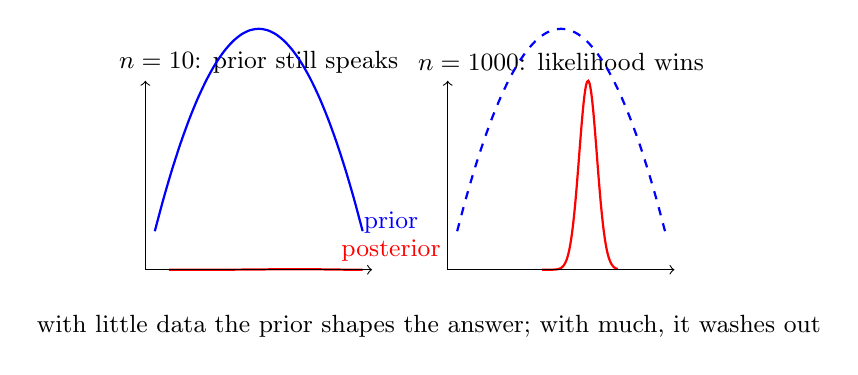
\begin{tikzpicture}[scale=0.6]
\begin{scope}
\node at (2.4,4.4) {\small $n=10$: prior still speaks};
\draw[domain=0.2:4.6,smooth,thick,blue] plot (\x,{3.4*(\x/4.8)*(1-\x/4.8)*6});
\draw[domain=0.5:4.6,smooth,thick,red,samples=50] plot (\x,{24*((\x/4.8)^8*(1-\x/4.8)^4)});
\draw[->] (0,0)--(4.8,0); \draw[->] (0,0)--(0,4);
\end{scope}
\begin{scope}[xshift=6.4cm]
\node at (2.4,4.4) {\small $n=1000$: likelihood wins};
\draw[domain=0.2:4.6,smooth,thick,blue,dashed] plot (\x,{3.4*(\x/4.8)*(1-\x/4.8)*6});
\draw[domain=2.0:3.6,smooth,thick,red,samples=60] plot (\x,{4.0*exp(-((\x-2.97)^2)/0.07)});
\draw[->] (0,0)--(4.8,0); \draw[->] (0,0)--(0,4);
\end{scope}
\node[blue] at (5.2,1.0) {\small prior};
\node[red] at (5.2,0.4) {\small posterior};
\node at (6.0,-1.2) {\small with little data the prior shapes the answer; with much, it washes out};
\end{tikzpicture}

\caption{Likelihood vs.\ posterior at two data sizes. Notice at $n=10$
the prior still visibly bends the answer; at $n=1000$ the likelihood
wins --- this is the honest version of ``the data speaks''.
Regenerate: \ttfamily figures/ch13\_lik\_vs\_post.tex.}
\label{fig:likpost}
\end{figure}

\begin{exercise}[medium]
Why is the posterior not just the likelihood normalized?
\begin{solution}
The prior multiplies in first: posterior $\propto$ likelihood $\times$
prior. Normalizing the likelihood alone discards the prior's weighting
--- that's MLE with extra steps, not Bayes.
\end{solution}
\end{exercise}

\section{MAP vs.\ MLE}\label{sec:stats-map}

\emph{Maximum a posteriori}\index{MAP} estimation takes the posterior's
mode: $\hat\theta_{\mathrm{MAP}}=\arg\max\,p(\theta)\,L(\theta)$ ---
MLE with a regularizer built in. When the prior is flat, MAP$=$MLE; when
data is thin, MAP stays sensible where MLE overfits (a Beta$(2,2)$ prior
on one flip keeps the answer off the rails). Ridge regression is MAP
with a Gaussian prior --- chapter 14's regularization is this section in
disguise.

\section{Regression revisited: least squares = MLE}\label{sec:stats-ls}

Model $y_i=\mathbf w^{T}\mathbf x_i+\varepsilon_i$ with
$\varepsilon_i\sim N(0,\sigma^{2})$ iid. Then
\[
L(\mathbf w)\propto\exp\!\Big(-\tfrac{1}{2\sigma^{2}}
\sum_i(y_i-\mathbf w^{T}\mathbf x_i)^{2}\Big)
\Rightarrow \ell=-\mathrm{const}-\tfrac{1}{2\sigma^{2}}\lVert\mathbf
y-X\mathbf w\rVert^{2}:
\]
maximizing likelihood = minimizing squared error. Chapter 8's least
squares was a statistical estimator all along --- the Gaussian-noise
assumption was hiding in the squaring.

\begin{example}[Deriving the logistic-regression NLL]\label{ex:logitnll}
\textbf{Strategy.} Binary $y\in\{0,1\}$, model
$\Pr[y=1\mid\mathbf x]=\sigma(\mathbf w^{T}\mathbf x+b)$,
$\sigma(z)=1/(1+e^{-z})$. The likelihood is a Bernoulli product; take
$-\log$.

\textbf{Solution.}
$\mathrm{NLL}=-\sum_i[y_i z_i-\log(1+e^{z_i})]$,
$z_i=\mathbf w^{T}\mathbf x_i+b$ --- written in the stable form
$\sum_i[\log(1+e^{z_i})-y_i z_i]$ = the listing's
\texttt{logaddexp}. Convex, no closed-form minimum, ready for
gradient descent in chapter 14 (Figure~\ref{fig:sigmoid}).
\end{example}

\begin{figure}[htbp]
\centering
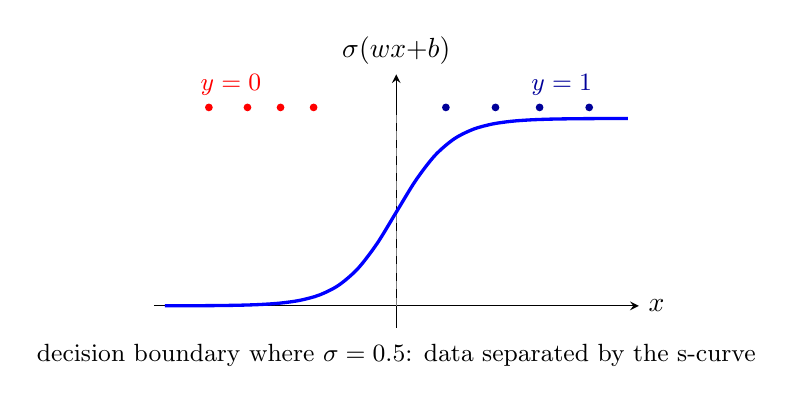
\begin{tikzpicture}[scale=0.7,>=stealth]
\draw[->] (-4.4,0)--(4.4,0) node[right]{$x$};
\draw[->] (0,-0.4)--(0,4.2) node[above]{$\sigma(wx{+}b)$};
\draw[domain=-4.2:4.2,smooth,very thick,blue] plot (\x,{3.4/(1+exp(-2*\x))});
\foreach \x in {-3.4,-2.7,-2.1,-1.5} \fill[red] (\x,3.6) circle (2pt);
\foreach \x in {0.9,1.8,2.6,3.5} \fill[blue!60!black] (\x,3.6) circle (2pt);
\draw[dashed,gray] (0,0)--(0,3.6);
\node[red] at (-3.0,4.0) {\small $y=0$};
\node[blue!60!black] at (3.0,4.0) {\small $y=1$};
\node at (0,-0.9) {\small decision boundary where $\sigma=0.5$: data separated by the s-curve};
\end{tikzpicture}

\caption{The logistic sigmoid and a 1-D decision boundary. Notice the
probabilities compress toward $0$/$1$ --- the decision boundary sits
where $\sigma=0.5$. Regenerate: \ttfamily figures/ch13\_sigmoid.tex.}
\label{fig:sigmoid}
\end{figure}

\begin{lstlisting}[caption={\ttfamily code/ch13\_logistic\_nll.py ---
the logistic NLL convexity-checked and grid-minimized: tomorrow's loss
landscape, today.}]
import numpy as np
np.set_printoptions(precision=4, suppress=True)
rng = np.random.default_rng(3)
# 1-D logistic regression data
x = rng.normal(0, 1, 40)
y = (x + rng.normal(0, 0.9, 40) > 0).astype(float)
def nll(w, b):
    z = w*x + b
    return np.sum(np.logaddexp(0, z) - y*z)   # stable NLL
# convexity check: NLL midpoint <= average (Jensen on 200 random pairs)
bad = 0
for _ in range(200):
    w1,b1 = rng.normal(0,3,2); w2,b2 = rng.normal(0,3,2)
    if nll((w1+w2)/2,(b1+b2)/2) > (nll(w1,b1)+nll(w2,b2))/2: bad += 1
print("convexity violations:", bad, "/200")
# numeric minimum by grid
W, B = np.meshgrid(np.linspace(-5,5,101), np.linspace(-5,5,101))
Z = np.zeros_like(W)
for i in range(W.shape[0]):
    for j in range(W.shape[1]): Z[i,j] = nll(W[i,j], B[i,j])
i,j = np.unravel_index(Z.argmin(), Z.shape)
print("grid minimum NLL %.3f at w=%.2f b=%.2f" % (Z[i,j], W[i,j], B[i,j]))
\end{lstlisting}

\begin{lstlisting}[caption={Output of the logistic experiment. Notice
0/200 Jensen violations --- the NLL surface is empirically convex, which
is why gradient descent will work on it in chapter 14.}]
convexity violations: 0 /200
grid minimum NLL 18.376 at w=2.00 b=-0.40
\end{lstlisting}

\begin{exercise}[easy]
Why minimize $-\ell$ rather than maximize $L$ numerically?
\begin{solution}
Raw $L$ underflows: $0.7^{700}\approx10^{-108}$ is borderline, and real
datasets kill it outright. Logs turn products into sums and keep the
objective in range.
\end{solution}
\end{exercise}

\begin{exercise}[hard]
Show ridge regression's $\lambda\lVert\mathbf w\rVert^{2}$ penalty is a
Gaussian prior $N(0,\tau^{2}I)$ on $\mathbf w$ under MAP --- identify
$\tau$ in terms of $\lambda,\sigma^{2}$.
\begin{solution}
$\ell_{\mathrm{MAP}}=-\frac{1}{2\sigma^2}\lVert y-Xw\rVert^2
-\frac{1}{2\tau^2}\lVert w\rVert^2+\mathrm{const}$; matching
$\lambda\lVert w\rVert^2$ gives $\tau^2=\sigma^2/\lambda$ ---
regularization strength is prior tightness.
\end{solution}
\end{exercise}

\section{Hand derivation}\label{sec:handderiv13}

Gaussian MLE in full. With $x_1,\dots,x_n$ iid $N(\mu,\sigma^{2})$:
\[
\ell(\mu,\sigma^{2})=-\frac{n}{2}\log(2\pi)
-\frac{n}{2}\log\sigma^{2}-\frac1{2\sigma^{2}}\sum_i(x_i-\mu)^{2}.
\]
$\partial\ell/\partial\mu=\frac1{\sigma^{2}}\sum_i(x_i-\mu)=0
\Rightarrow\hat\mu=\bar x$. For $\sigma^{2}$ write $v=\sigma^{2}$:
$\partial\ell/\partial v=-\frac{n}{2v}+\frac{1}{2v^{2}}\sum_i
(x_i-\mu)^{2}=0\Rightarrow\hat\sigma^{2}=\frac1n\sum_i(x_i-\bar x)^{2}$.
The bias: $\mathbb E[\hat\sigma^{2}]=\frac{n-1}{n}\sigma^{2}$ ---
one degree of freedom went to estimating $\mu$ first; the unbiased fix
divides by $n-1$, verified in the listing.

\section{Common mistakes}\label{sec:stats-mistakes}

\begin{tripwire}[{Maximizing raw likelihood numerically}]
$L(\theta)$ for 1000 Bernoulli trials is $\sim10^{-300}$ at best ---
float64 reads it as zero and every optimizer stalls. Always work in
log-likelihood.
\end{tripwire}

\begin{tripwire}[{MLE vs.\ MAP conflated}]
MLE maximizes $L$; MAP maximizes $L\times$prior. They agree only under
flat priors or infinite data --- saying ``the MLE'' when a prior was
used hides an assumption.
\end{tripwire}

\begin{tripwire}[{Dividing by $n$ vs.\ $n-1$ without knowing why}]
$n$ gives the MLE (biased low, variance-squeezed); $n-1$ gives the
unbiased estimator. The listing shows both exactly --- pick on purpose,
not by habit.
\end{tripwire}

\begin{tripwire}[{Treating a point estimate as the posterior}]
$\hat\theta$ is one coordinate of the posterior, not the posterior.
Only the full distribution supports ``how sure are we'' questions ---
a Beta $(720,394)$ answer and a Beta $(2,2)$ answer may share a mean.
\end{tripwire}

\begin{tripwire}[{Likelihood as a probability over $\theta$}]
$L(\theta)$ need not integrate to 1 over $\theta$ --- it is a
probability over DATA, indexed by $\theta$. Integrating it as if it were
a posterior is the prosecutor's fallacy in analytic form.
\end{tripwire}

\section{Summary}

\begin{center}
\begin{tabularx}{\textwidth}{l>{\raggedright\arraybackslash}X}
\toprule
\textbf{Object} & \textbf{What you need to know}\\
\midrule
Estimator & a statistic aimed at a parameter; has a sampling
distribution \\
MSE decomposition & var $+$ bias$^{2}$ --- the trade-off behind every
fit \\
Likelihood & $L(\theta)=p(\text{data}\mid\theta)$; maximize in LOGS ---
underflow otherwise \\
MLEs to know & coin $\to H/n$; Gaussian $\to(\bar x,\frac1n\sum_{i=1}^{n}
(x_i-\bar x)^2)$ (biased!) \\
Bayesian & posterior $\propto$ likelihood$\times$prior; Beta+binomial
conjugate: just add counts \\
MAP & posterior mode; flat prior $\Rightarrow$ MAP$=$MLE; Gaussian
prior $\Rightarrow$ ridge \\
LS as MLE & Gaussian noise: $\min\|y-Xw\|^2$ IS $\max L$; logistic NLL
$=\sum_{i=1}^{n}[\log(1+e^{z_i})-y_iz_i]$ \\
\bottomrule
\end{tabularx}
\end{center}
\begin{rulebox}[{Watch instead}]
\begin{enumerate}
\item \emph{Maximum Likelihood, clearly explained!!!} --- StatQuest
with Josh Starmer, 6:12, \url{https://youtu.be/XepXtl9YKwc} ---
\S\ref{sec:stats-mle} in its shortest honest form
(accessed 2026-10-11).
\item \emph{Machine Learning Fundamentals: Bias and Variance} ---
StatQuest, 6:36, \url{https://youtu.be/EuBBz3bI-aA} ---
\S\ref{sec:stats-bv} (accessed 2026-10-11).
\item \emph{Logistic Regression Details Pt 2: Maximum Likelihood} ---
StatQuest, 10:23, \url{https://youtu.be/BfKanl1aSG0} ---
\S\ref{sec:stats-ls} the MLE-as-loss story (accessed 2026-10-11).
\end{enumerate}
\end{rulebox}

\section*{Further reading}
\addcontentsline{toc}{section}{Further reading}

\begin{itemize}
\item MIT OpenCourseWare, \emph{18.05 Introduction to Probability and
Statistics} --- the statistics half of this book's foundations, at OCW
(course ``18.05''), \url{https://ocw.mit.edu}. Verified 2026-10-11.
\item D.~Bertsekas and J.~Tsitsiklis, \emph{Introduction to
Probability}, 2nd ed., ch.~9 --- classical statistics from the
probabilist's side. ISBN 978-1886529236.
\item L.~Wasserman, \emph{All of Statistics}, chs.~6, 9 --- the
frequentist machinery (sampling distributions, MLE) in one
graduate-level reference. ISBN 978-0387402727.
\item M.~Deisenroth et al., \emph{Mathematics for Machine Learning},
\S8--9 (free PDF) --- parameter estimation and regression as
inference.\newline
\url{https://mml-book.github.io/book/mml-book.pdf}
Verified 2026-10-11.
\item C.~M.~Bishop, \emph{Pattern Recognition and Machine Learning},
\S1.2, \S4.3 --- Bayesian inference and the logistic-regression NLL.
ISBN 978-0387310732.
\item StatQuest channel playlists on estimation and classification ---
the video versions of this chapter's WEs.\newline
\url{https://www.youtube.com/@statquest/playlists}
Verified 2026-10-11.
\end{itemize}

\section*{Additional exercises}
\addcontentsline{toc}{section}{Additional exercises}

\begin{exercise}[easy]
Estimate the mean of $N(\mu,4)$ from samples $3,5,4,6,2$: compute
$\hat\mu$ and its standard error.
\end{exercise}

\begin{exercise}[easy]
Geometric$(p)$: derive the MLE of $p$ from $n$ iid trials.
\end{exercise}

\begin{exercise}[easy]
For the Beta$(2,2)$ prior, what single flip moves the posterior mean
most? Say why.
\end{exercise}

\begin{exercise}[easy]
Is $\bar x^{2}$ an unbiased estimator of $\mu^{2}$? Compute its bias.
\end{exercise}

\begin{exercise}[medium]
Poisson MLE: show $\hat\lambda=\bar x$ and that it is unbiased ---
one of the few MLEs that is.
\end{exercise}

\begin{exercise}[medium]
In code: repeat the sampling-distribution experiment at $n=30$; how do
bias and variance of the two variance estimators change? Report MSE of
each.
\end{exercise}

\begin{exercise}[medium]
Derive the MAP estimator for the coin with Beta$(a,b)$ prior; show it
interpolates between the prior mode and the MLE as $n\to\infty$.
\end{exercise}

\begin{exercise}[medium]
Show the sample median is a consistent estimator of a symmetric
distribution's center; compute its bias for 5-point Gaussian samples
numerically.
\end{exercise}

\begin{exercise}[medium]
Jeffreys prior $\mathrm{Beta}(\tfrac12,\tfrac12)$ vs.\ Laplace's
$\mathrm{Beta}(1,1)$: update both on 7H/3T and compare posterior means
--- how much does prior choice matter here?
\end{exercise}

\begin{exercise}[hard]
Prove $\mathbb E[\hat\sigma^{2}_{/n}]=\frac{n-1}{n}\sigma^{2}$ exactly:
expand $\sum_i(x_i-\bar x)^2=\sum_i(x_i-\mu)^2-n(\bar x-\mu)^2$ and take
expectations.
\end{exercise}

\begin{exercise}[hard]
Conjugate-prior derivation: show Gamma is conjugate for a Poisson
likelihood --- write the posterior's parameters after $n$ observations.
\end{exercise}

\begin{exercise}[hard]
Fisher information for the Bernoulli: compute
$I(\theta)=-\mathbb E[\ell''(\theta)]=n/(\theta(1-\theta))$ and connect
its reciprocal to the Cram\'er--Rao bound for $\hat\theta$.
\end{exercise}

\begin{exercise}[hard]
Implement rejection sampling for the Beta$(720,394)$ posterior of
Example~\ref{ex:betacoin}; verify the sampled mean/variance against the
analytic Beta moments.
\end{exercise}
\begin{exercise}[medium]
For the die of example~\ref{ex:sampdist}, find
$\operatorname{Var}(\bar X)$ with $n=16$ rolls, then use Chebyshev to
bound $P(|\bar X-3.5|\geq0.5)$. What sample size makes the bound
below $0.05$?
\end{exercise}
\begin{exercise}[hard]
Show $\hat\sigma^{2}=\frac1n\sum(X_i-\bar X)^{2}$ is biased: compute
$E[\hat\sigma^{2}]=\frac{n-1}{n}\sigma^{2}$ directly. Then find the
unbiased correction (Bessel's correction) and explain the $n-1$
geometrically (the residuals live in an $(n-1)$-dimensional subspace).
\end{exercise}

\chapternotes{%
The estimator-framework and the MLE worked set follow MML \S6.4--6.5,
ch.~9 \cite{mml}; the Bayesian-inference-before-regression ordering
follows MIT 18.05 \cite{ocw1805}; the story-first register of the
estimation sections follows Blitzstein \& Hwang \cite{stat110}; the
classical-vs-Bayesian split follows Pishro-Nik \cite{pishronik}. All
simulations seeded; printed blocks are this box's real output.}
